%------------------------------------------------------------------------------
% Opções das classes-padrão (article, book e report)
%
% Tamanho da fonte:
%   10pt (padrão)
%   11pt
%   12pt
%
% Tamanho do papel:
%   letterpaper (padrão)
%   legalpaper
%   executivepaper
%   a4paper
%   a5paper
%   b5paper
%
% Orientação da página:
%   portraid (padrão)
%   landscape
%
% Colunas:
%   onecolumn (padrão)
%   twocolumn
%
% Impressão:
%   oneside (padrão em article e report)
%   twoside (padrão na book)
%
% Abertura de capítulos:
%   openright (padrão)
%   openany
%
% Capa:
%   titlepage (padrão em book e report)
%   notitlepage (padrão em article)
%
% Posição das expressões matemáticas:
%   fleqn
%
% Posição dos números das expressões matemáticas:
%   leqno
%
% Auxiliar:
%   final (padrão)
%   draft
%------------------------------------------------------------------------------
\documentclass[a4paper,12pt]{book}
%\documentclass[a4paper,12pt]{scrbook} % <-- Faz parte do "bundle" Koma-Script

	\usepackage[ansinew]{inputenc}		
	\usepackage[brazil]{babel}
	
	%----------------------------------------------------------------------------
	% Utilize o pacote hyperref para criar links automaticamente no seu documento
	% e um bookmark. MAS APENAS SE VOCÊ ESTIVER COMPILANDO PARA GERAR UM PDF!
	%----------------------------------------------------------------------------
	\usepackage{hyperref}
	
	%----------------------------------------------------------------------------
	% Promove a endentação do primeiro parágrafo de uma seção.
	%----------------------------------------------------------------------------
	\usepackage{indentfirst}
	
	%----------------------------------------------------------------------------
	% Outra família de fontes: utopia (inclusive para modo matemático).
	%----------------------------------------------------------------------------
	\usepackage{ae} % <-- No lugar do pacote "ae"
	
	%----------------------------------------------------------------------------
	% O pacote tikz define inúmeros comandos para desenhos vetoriais. Utilize-o
	% aqui apenas para ilustrar o ambiente titlepage, logo mais.
	%----------------------------------------------------------------------------
	\usepackage{tikz}
	
	%----------------------------------------------------------------------------
	% Dois pacotes auxiliares que você já conhece.
	%----------------------------------------------------------------------------
	%\usepackage{layout}
	\usepackage{lipsum}
	
	%----------------------------------------------------------------------------
	% No caminho para as suas figuras, você pode utilizar o ponto-final . para
	% denotar a pasta atual e .. para denotar a pasta imediatamente acima.
	%----------------------------------------------------------------------------
	\usepackage{graphicx}
	\graphicspath{{./figuras/}}
	
	%----------------------------------------------------------------------------
	% O pacote "fancyhdr" oferece muito mais flexibilidade de configuração do 
	% cabeçalho e rodapé que os comandos padrão do LaTeX. Portanto, recomendamos
	% que você o utilize, salvo em situações excepcionalmente simples, como 
	% remover a numeração de páginas apenas (neste caso a instrução 
	% \pagestyle{empty} é suficiente e nenhum pacote adicional, requerido). As
	% letras utilizadas no argumento opcional dos comandos \fancyhead e 
	% \fancyfoot representam o seguinte:
	% E: páginas pares (even pages)
	% O: páginas ímpares (odd pages)
	% L: esquerda (left)
	% C: centro (center)
	% R: direita (right)
	%----------------------------------------------------------------------------
	\usepackage{fancyhdr}
	
	\pagestyle{fancy}
	\fancyhead{} % <-- Limpa o cabeçalho.
	\fancyhead[LE]{\raisebox{0pt}[0pt][0pt]{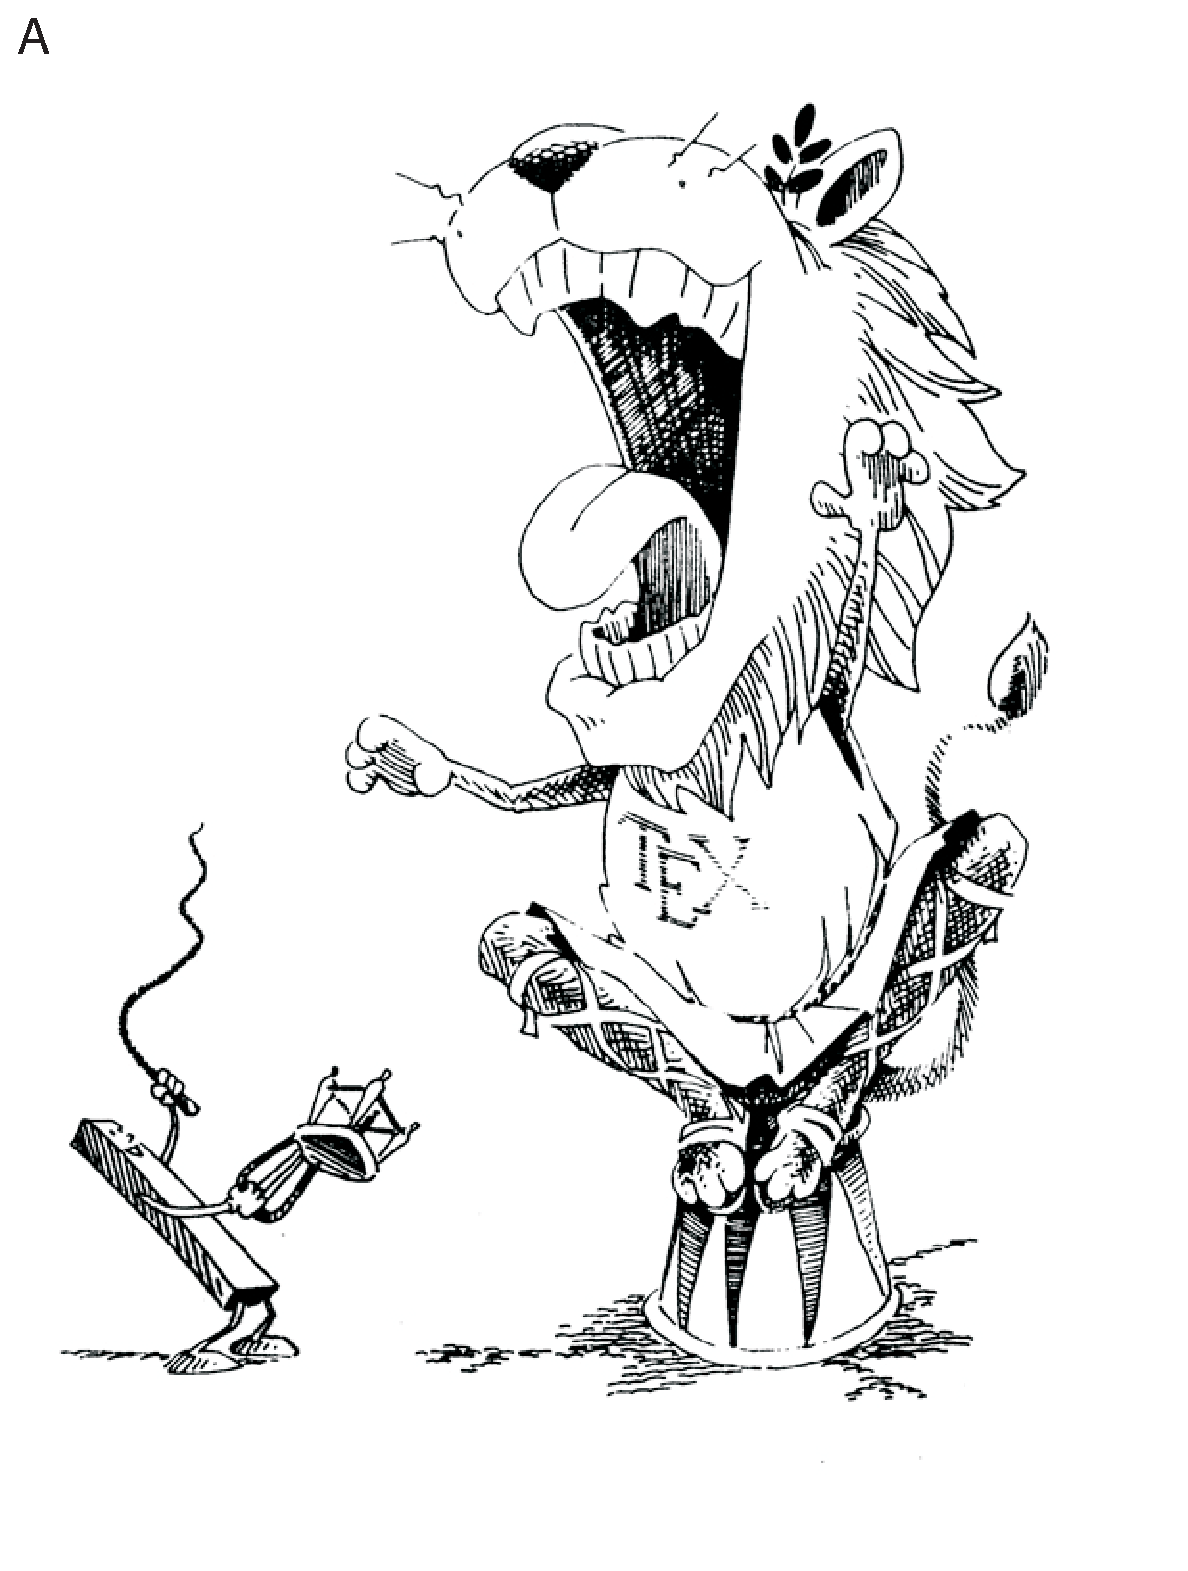
\includegraphics[height=\headheight]{Controlling_TeX}}}
	\fancyhead[RO]{\foreign{Right of odd pages}}	
	\fancyfoot{} % <-- Limpa o rodapé.
	\fancyfoot[RO,LE]{\thepage} % <-- Número da página à direita em páginas 
	                            %     ímpares e à esquerda nas pares.
	%----------------------------------------------------------------------------
	% A redefinição da espessura das linhas de cabeçalho e rodapé parece ser meio
	% patológica. Isto é, o correto seria definir \headrulewidth e \footrulewidth
	% (abaixo) como comprimentos ao invés de comandos. Mas aparentemente o desen-
	% volvedor do pacote não pensou assim. Por isso, para controlar essas 
	% espessuras você deve utilizar \renewcommand ao invés de \setlength.
	%----------------------------------------------------------------------------
	\renewcommand{\headrulewidth}{1pt}
	\renewcommand{\footrulewidth}{1pt}
	
	%----------------------------------------------------------------------------
	% Os comandos \headrule e \footrule SÃO as linhas propriamente ditas, que
	% utilizam os parâmetros \headrulewidth e \footrulewidth acima. Mas eu posso
	% redefiní-lo completamente, como abaixo, onde eu decidi trocar a linha de
	% cabeçalho por uma linha dupla. obs.: o comando \llap (left overlap) traz
	% seu argumento (uma caixa) para cima da caixa imediatamente anterior. Peça
	% ao professor para explicar isto. Existe também o \rlap (right overlap).
	%----------------------------------------------------------------------------
%	\renewcommand{\headrule}{
%		\raisebox{1.5pt}{\rule{\textwidth}{0.1pt}}%
%		\llap{\rule{\textwidth}{0.1pt}}}
	
	%----------------------------------------------------------------------------
	% O comando \input abaixo insere o arquivo defs.tex nesta posição, como se 
	% todo o conteúdo daquele arquivo tivesse sido digitado aqui. Particularmente
	% neste caso, o arquivo defs.tex contém algumas definições de comandos 
	% utilizadas aqui.
	%----------------------------------------------------------------------------
	%-------------------------------------------------------------------------
% Ao inv�s de inserir o arquivo usandoLaTeX.tex com suas pr�prias defini��es
% de comandos atrav�s do \input, voc� pode definir seu pr�prio pacote! Para
% isto, basta trocar os \usepackage (do arquivo usandoLaTeX.tex) por
% \RequirePackage e colocar, no come�o do arquivo, o comando
% \ProvidesPackage{NOME}, onde NOME � o nome do seu pacote, que deve coincidir
% com o do arquivo (mais a extens�o "sty", de style): NOME.sty.
%-------------------------------------------------------------------------
\ProvidesPackage{usandoLaTeX}

%-------------------------------------------------------------------------
% Ao inv�s do usual \usepackage, utilize \RequirePackage para informar ao
% LaTeX quais pacotes voc� precisa para definir seus pr�prios comandos. A
% sintaxe deste comando � id�ntica � do \usepackage.
%-------------------------------------------------------------------------
\RequirePackage{xspace,xcolor,ifthen}

%-------------------------------------------------------------------------
% Finalmente, seus comandos. Lembre-se: definir seus pr�prios comandos �
% o que o(a) permitir� explorar todo o potencial do LaTeX. DEFINA SEUS
% COMANDOS SEM D�!
%-------------------------------------------------------------------------
%\newcommand{\cs}[1]{{\normalfont\ttfamily\color{blue!50!black}\textbackslash #1}}
\newcommand{\cs}[2][\null]{%
	\normalfont{\color{blue!50!black}\textbackslash #2}%
	\ifthenelse{\equal{#1}{\null}}{}{\{#1\}}}
\newcommand{\pkg}[1]{{\normalfont\sffamily\color{green!50!white}#1}}
\newcommand{\cls}[1]{{\normalfont\sffamily\color{green!50!black}#1}}
\newcommand{\ctr}[1]{{\normalfont\sffamily\color{yellow!50!white}#1}}
\newcommand{\env}[1]{{\normalfont\sffamily\color{yellow!50!black}#1}}
\newcommand{\opt}[1]{{\normalfont\ttfamily\color{green!50!black}#1}}
\newcommand{\fntattr}[1]{{\normalfont\ttfamily #1}}
\newcommand{\foreign}[1]{\textsl{#1}}

\newcommand{\etc}{etc\xspace}
\newcommand{\ie}{ie\xspace}
\newcommand{\etal}{et~al\xspace}

\newcounter{obs}
\newcommand\obs{\stepcounter{obs}\textbf{obs.~\theobs:}\ }
	%\usepackage{usandoLaTeX}
		
	%----------------------------------------------------------------------------
	% O comando \title define o título do trabalho, mas NÃO o imprime (isto é
	% feito pelo comando \maketitle, mais a frente).
	%----------------------------------------------------------------------------
	\title{O título deste trabalho}
	
	%----------------------------------------------------------------------------
	% O comando \author define o(s) autor(es) do trabalho. Cada autor deve ser
	% separado pela instrução \and. O comando \thanks insere uma nota de rodapé,
	% gealmente utilizada (neste contexto) para informar e-mails.
	%----------------------------------------------------------------------------

	\author{
		Fulano de tal\thanks{fulano@latex.br}\\
		Instituto dos fulaninhos
		\and
		Sicrano de tal\thanks{sicrano@tex.br}\\
		Universidade dos sicraninhos}
		
	%----------------------------------------------------------------------------
	% O comando \date define a data do trabalho. Você pode escrevê-la no formato
	% que quiser ou omití-lo. Neste caso, o LaTeX inserirá automaticamente a data
	% atual no formato padrão (não se esqueça de utilizar o pacote babel ou ela
	% será apresentada no formato americano).
	%----------------------------------------------------------------------------
	\date{São Paulo, \today}
	
	% Metadados do arquivo PDF.
	\hypersetup{
		pdftitle={Exemplo de uso de classes para livros},
		pdfauthor={Dr. Ivan R. Pagnossin},
		pdfsubject={LaTeX},
		pdfkeywords={TeX,LaTeX}
	}
	
\begin{document}
		
	%----------------------------------------------------------------------------
	% O comando \frontmatter, quando presente, marca o início do conteúdo que 
	% antecede o trabalho propriamente dito. É onde você colocará o sumário,
	% prefácio, dedicatória, agradecimentos, listas de figuras, de tabelas, etc.
	%----------------------------------------------------------------------------
	\frontmatter
			
	%----------------------------------------------------------------------------
	% O comando \maketitle organiza (imprime) os dados que você forneceu através
	% dos comandos \title, \author e \date. Isto é, estes três comandos são
	% declarações: não produzem nada, mas influem no lhes sucedem: o resultado
	% do comando \maketitle.
	%----------------------------------------------------------------------------
	\maketitle
	
	%----------------------------------------------------------------------------
	% Alternativamente ao \maketitle, você pode criar sua própria capa. Neste
	% caso, você não deve utilizar o \maketitle, e os comandos \title, \author e
	% \date perdem a utilidade.
	%----------------------------------------------------------------------------
%	\begin{titlepage}
%	
%		%--------------------------------------------------------------------------
%		% Para utilizar este ambiente você deve carregar o pacote tikz.
%		%--------------------------------------------------------------------------
%		\begin{tikzpicture}[remember picture,overlay]
%			\node [opacity=0.25] at (current page.center) 		
%			{\includegraphics[height=\paperheight,width=\paperwidth]{DonaldEKnuth}};
%		\end{tikzpicture}
%			
%		\vfill
%	
%		\centering\Huge
%		O título deste trabalho\\
%		Fulano \& Sicrano
%		
%		\vfill
%		
%	\end{titlepage}
		
	%----------------------------------------------------------------------------
	% O comando \tableofcontents insere no documento o sumário ("table of 
	% contents"). O LaTeX faz isso automaticamente com base nos comandos de
	% capítulo, seções, etc.
	%----------------------------------------------------------------------------
	\tableofcontents
	
	%----------------------------------------------------------------------------
	% O comando \listoffigures insere no documento a lista de figuras utilizadas,
	% mas apenas aquelas dentro do ambiente "figure". Isto porque é este ambiente
	% que modifica o contador "figure" (o comando \caption, para ser mais exato),
	% que é utilizado para construir a lista de figuras.
	%----------------------------------------------------------------------------
	%\listoffigures
		
	%----------------------------------------------------------------------------
	% O comando \listoftables insere no documento a lista de tabelas utilizadas,
	% mas apenas aquelas dentro do ambiente "table". Isto porque é este ambiente
	% que modifica o contador "table" (o comando \caption, para ser mais exato),
	% que é utilizado para construir a lista de tabelas.
	%----------------------------------------------------------------------------
	%\listoftables
	
	\chapter{Prefácio}
	
	O comando \cs{chapter}, disponível nas classes \cls{book} e \cls{report}, 
	marca o início de um capítulo. Com um detalhe: aqui ele ainda está sob a
	influência da declaração \cs{frontmatter} e, por isso, não tem um número 
	associado a ele.\footnote{Na verdade, ocorre que o contador associado ao
	comando \cs{chapter} (de nome \ctr{chapter}) permanece em zero, seu valor
	inicial.}
	
	%----------------------------------------------------------------------------
	% O comando \mainmatter, quando presente, marca o início do corpo do trabalho
	% propriamente dito. Este é o estado padrão do documento. Isto é, se você não
	% utilizar \frontmatter, \mainmatter ou \backmatter (a seguir), o LaTeX 
	% assumirá que todo o conteúdo no ambiente "document" faz parte do corpo do
	% documento (mainmatter).
	%----------------------------------------------------------------------------
	\mainmatter
	\chapter{Título deste capítulo}\label{chap:intro}
	
	O comando \cs{mainmatter}, quando presente, marca o início do corpo do
	trabalho propriamente dito. Este é o estado padrão do documento. Isto é, se
	você não utilizar \cs{frontmatter}, \cs{mainmatter} ou \cs{backmatter} (a
	seguir), o \LaTeX\ assumirá que todo o conteúdo no ambiente \env{document}
	faz	parte do corpo do	documento (mainmatter).	
	
	Observe que o comando \cs{chapter} não define apenas a forma como o título é
	exibido. Ele permite também a utilização do comando \cs{label}, para
	referências cruzadas, e inclui o título no sumário (ou \foreign{bookmarks},
	no caso de um documento PDF).
	
	%-------------------------------------------------------------------------
	\section{Esta é uma seção do capítulo \ref{chap:intro}}
		\label{sec:sec}
		
	É interessante observar que o \LaTeX\ não endenta o primeiro parágrafo de 
	cada seção, mesmo que você o instrua explicitamente a fazê-lo (com o comando
	\cs{indent}; oposto de \cs{noindent}). A maneira mais simples (e recomendada)
	de contornar este comportamento é utilizar o pacote \pkg{indentfirst}.
	
	%-------------------------------------------------------------------------
	\subsection*{Uma seção sem número e que não aparece no sumário}
		
	A versão com asterisco do comando \cs{subsection} inibe tanto a numeração
	como a presença da seção no sumário. Esta versão existe também para
	\cs{chapter},	\cs{section} e \cs{subsubsection} (este último, apenas nas
	classes	\cls{article} e \cls{report}).
		
	%-------------------------------------------------------------------------
	\section[Título alternativo]{Por alguma razão não nos interessa colocar todo
	este título no sumário}
		
	Ao iniciar uma seção, às vezes pode ser necessário inserir um nome
	alternativo	no sumário. Isto ocorre, por exemplo, quando o título da seção é
	demasiadamente longo, como aqui. Neste caso, passamos o nome alternativo ao
	comando \cs{section} na forma de um argumento opcional, \ie, entre colchetes.
	
	%-------------------------------------------------------------------------
	\paragraph{\S1\textordmasculine}
	
	Observe que o texto imediatamente após o comando \cs{paragraph} faz parte do
	parágrafo iniciado por ele.
	
	%-------------------------------------------------------------------------
	\subparagraph{\P} Idem para \cs{subparagraph}, mas atenção ao espaço vertical
	inerente a estes comandos.
	
	\section{Lorem ipsum}
	\lipsum[1-10]
	
	%-------------------------------------------------------------------------
	% A declaração \appendix marca o início dos apêndices. A partir daqui, todo
	% \chapter dará origem a um novo apêndice, cuja numeração será geralmente
	% em letras maiúsculas.
	\appendix
	\chapter{Montando apêndices}
	
	\section{A declaração \cs{appendix}}
	
	A declaração \cs{appendix} informa ao \LaTeX\ que os capítulos e seções
	\emph{iniciados} a	partir dali são apêndices do trabalho. É também nesta
	região que geralmente são incluídas as referências bibliográficas, o índice
	remissivo \etc.
	
	%-------------------------------------------------------------------------
	\section{O ambiente \env{appendix}}
	
	Alternativamente à declaração \cs{appendix}, você pode utilizar o ambiente
	\env{appendix},	o que pode ser útil para construir apêndices de capítulos
	isolados, por	exemplo.

	%-------------------------------------------------------------------------
	% A bibliografia não aparece automaticamente no sumário (lembre-se: trata-
	% se de uma lista apenas); você tem de inserí-la manualmente. Para isso,
	% utilize o comando \addcontentsline, como abaixo: "toc" indica que você
	% quer inserir esta informação no sumário ("table of contents"). "chapter"
	% indica a hierarquia da seção, ie, se se trata de um capítulo, de uma
	% seção, subseção, etc (no caso da bibliografia é quase certo que você
	% usará sempre "chapter"). Finalmente "Bibliografia" é o texto que você
	% quer inserir no sumário.
	%-------------------------------------------------------------------------
	\addcontentsline{toc}{chapter}{Bibliografia}
	
	%-------------------------------------------------------------------------
	% Conforme vimos, o ambiente thebibliography é apenas uma lista cujos ítens
	% podem ser referenciados no texto com o comando \cite (ao invés de \ref).
	%-------------------------------------------------------------------------
	\begin{thebibliography}{0}
		\bibitem{kopka:1998} H. Kopka e P. W. Daly, \textsl{A guide to \LaTeX},
		Addison-Wesley, 1998.
	\end{thebibliography}

	%-------------------------------------------------------------------------
	% Experimente utilizar a opção "landscape" da classe e chame o comando
	% \layout (abaixo) para exibir as dimensões envolvidas. Não se esqueça de
	% carregar o pacote layout, que define o comando \layout.
	%-------------------------------------------------------------------------
	%\layout

\end{document}